\documentclass[10pt]{article}
\usepackage[utf8]{inputenc}
\usepackage{listings}
\usepackage{float}
\usepackage{graphicx}
\usepackage{fullpage}
\usepackage{caption}
\usepackage{subcaption}
\usepackage{amsmath}
\usepackage{hyperref}

%\renewcommand{\thesubsection}{\arabic{subsection}}
\renewcommand{\thesubsubsection}{\alph{subsubsection}}

\title{Pattern Recognition Practical 5}
\author{Group 24: \and Maikel Withagen (s1867733) \and Steven Bosch (s1861948)}
\date{\today}
\lstset{
frame=single, 
numbers=left, 
breaklines=true, 
language=Matlab,
basicstyle=\footnotesize, 
title=\lstname,
showstringspaces=false
}

\DeclareMathOperator*{\argmax}{arg\!\max}

\renewcommand{\thesection}{Assignment \arabic{section}}
\renewcommand{\thesubsection}{\arabic{subsection}}
\begin{document}
\maketitle

\section{k-means clustering, quantization error, gap statistic}
\subsection{}
Using the code given in the Appendix(kmeans.m and runKMeans.m), 
we created the plots shown in figures \ref{fig1.1}, \ref{fig1.2} and \ref{fig1.3}.\\

\begin{figure}[H]
  \centering
  \caption{Results for k=2}
  \begin{subfigure}[b]{.45\textwidth}
    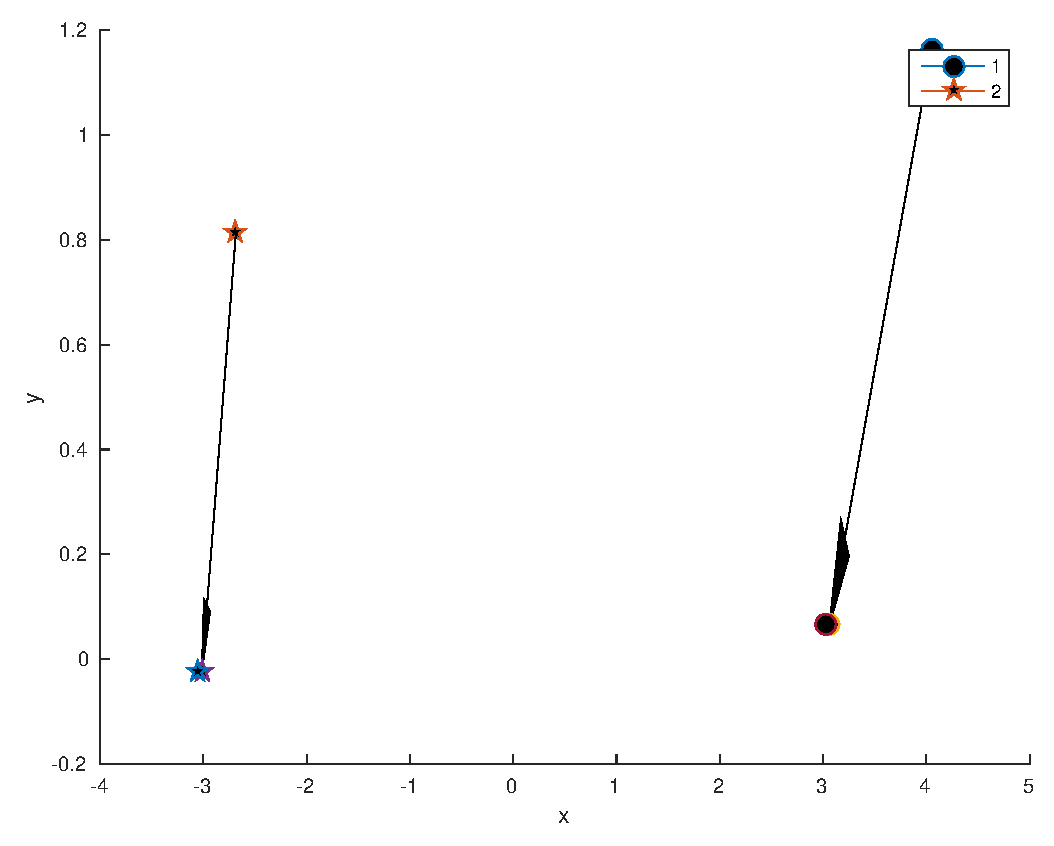
\includegraphics[width=\columnwidth]{Fig1_k2.eps}
    \caption{intermediate positions of the cluster means, 
    with their progress indicated by the arrows.}
    \label{fig1a}
  \end{subfigure}
  \quad
  \begin{subfigure}[b]{.45\textwidth}
    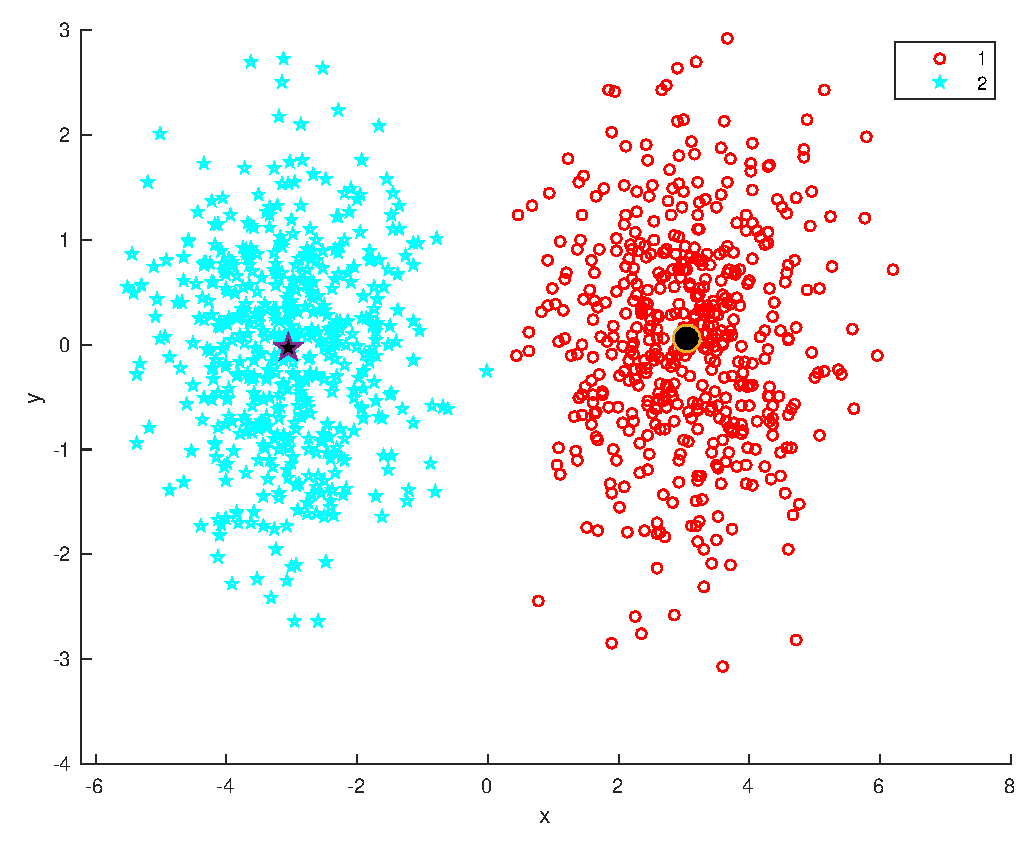
\includegraphics[width=\columnwidth]{Fig2_k2.eps}
    \caption{The final cluster means with their assigned data points)}
    \label{fig1b}
  \end{subfigure}
  \label{fig1.1}
\end{figure}

\begin{figure}[H]
  \centering
  \caption{Results for k=4}
  \begin{subfigure}[b]{.45\textwidth}
    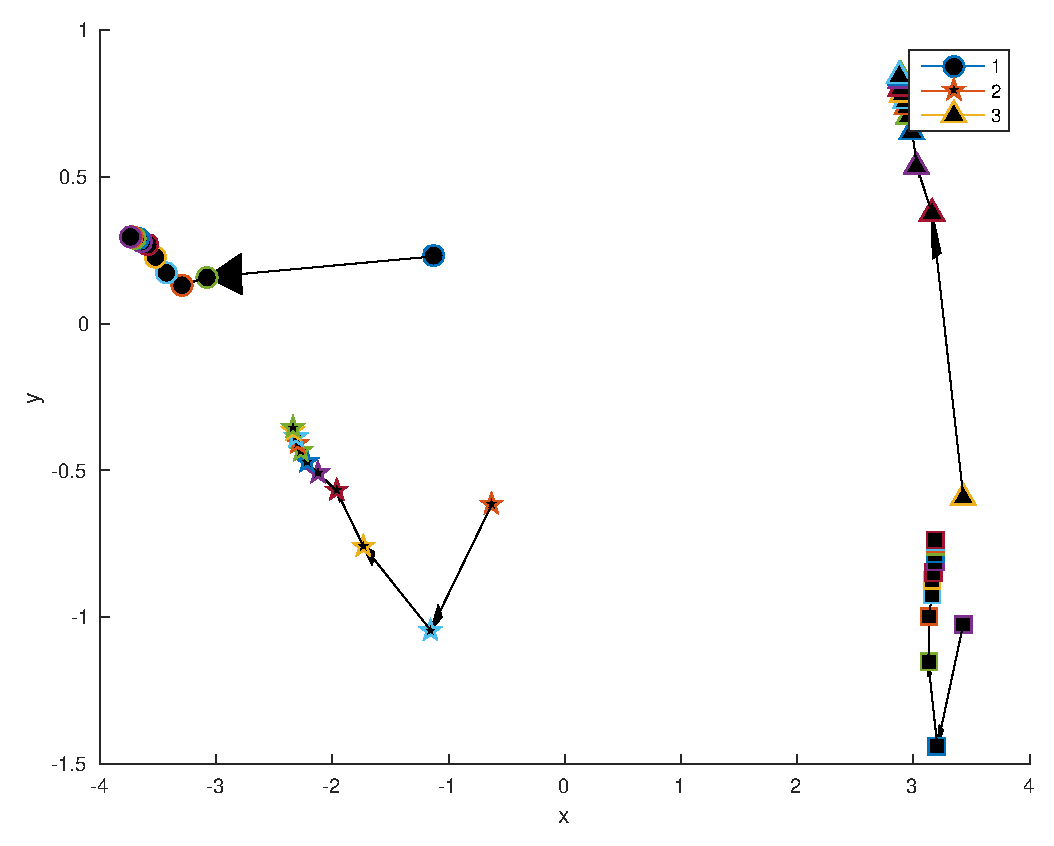
\includegraphics[width=\columnwidth]{Fig1_k4.eps}
    \caption{intermediate positions of the cluster means, 
    with their progress indicated by the arrows.}
  \end{subfigure}
  \quad
  \begin{subfigure}[b]{.45\textwidth}
    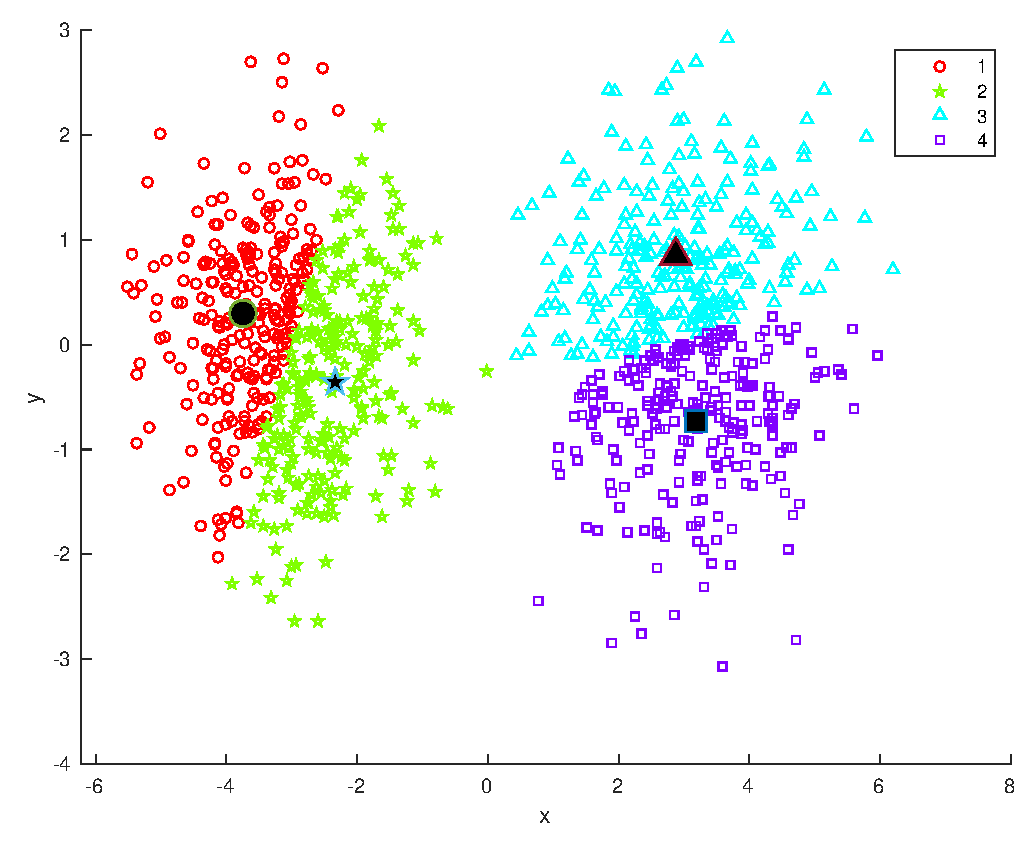
\includegraphics[width=\columnwidth]{Fig2_k4.eps}
    \caption{The final cluster means with their assigned data points)}
  \end{subfigure}
  \label{fig1.2}
\end{figure}

\begin{figure}[H]
  \centering
  \caption{Results for k=8}
  \begin{subfigure}[b]{.45\textwidth}
    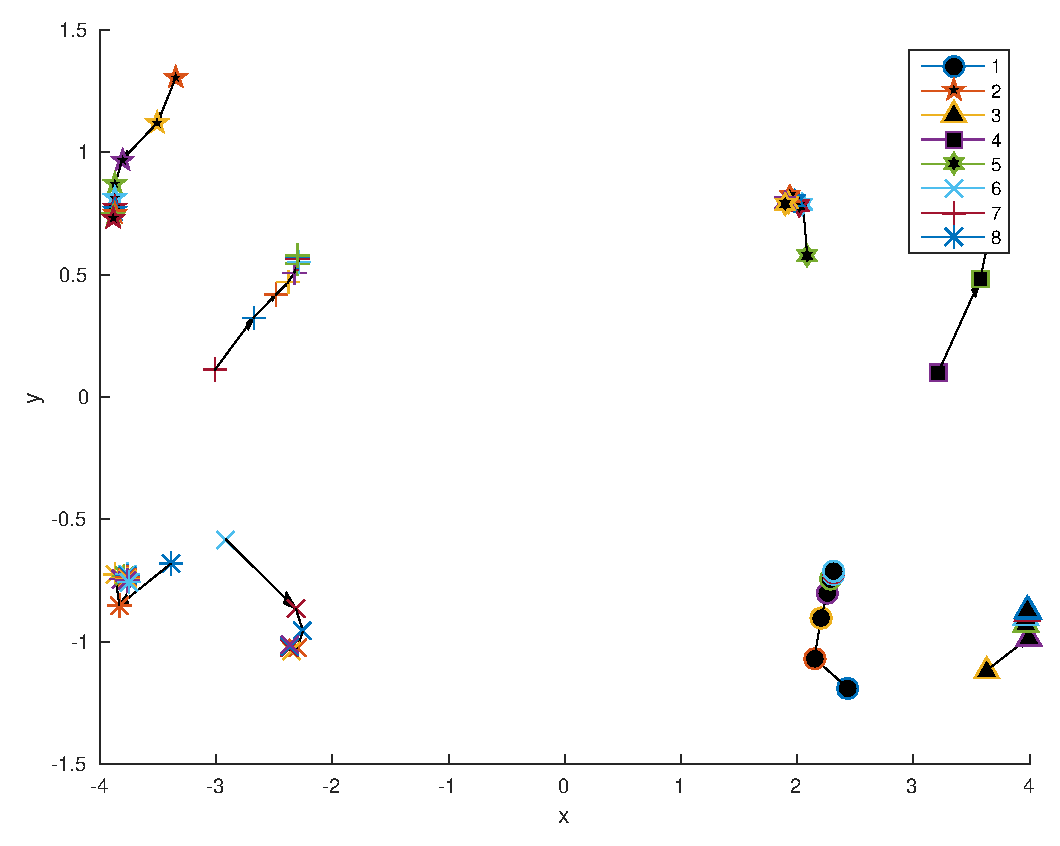
\includegraphics[width=\columnwidth]{Fig1_k8.eps}
    \caption{intermediate positions of the cluster means, 
    with their progress indicated by the arrows.}
  \end{subfigure}
  \quad
  \begin{subfigure}[b]{.45\textwidth}
    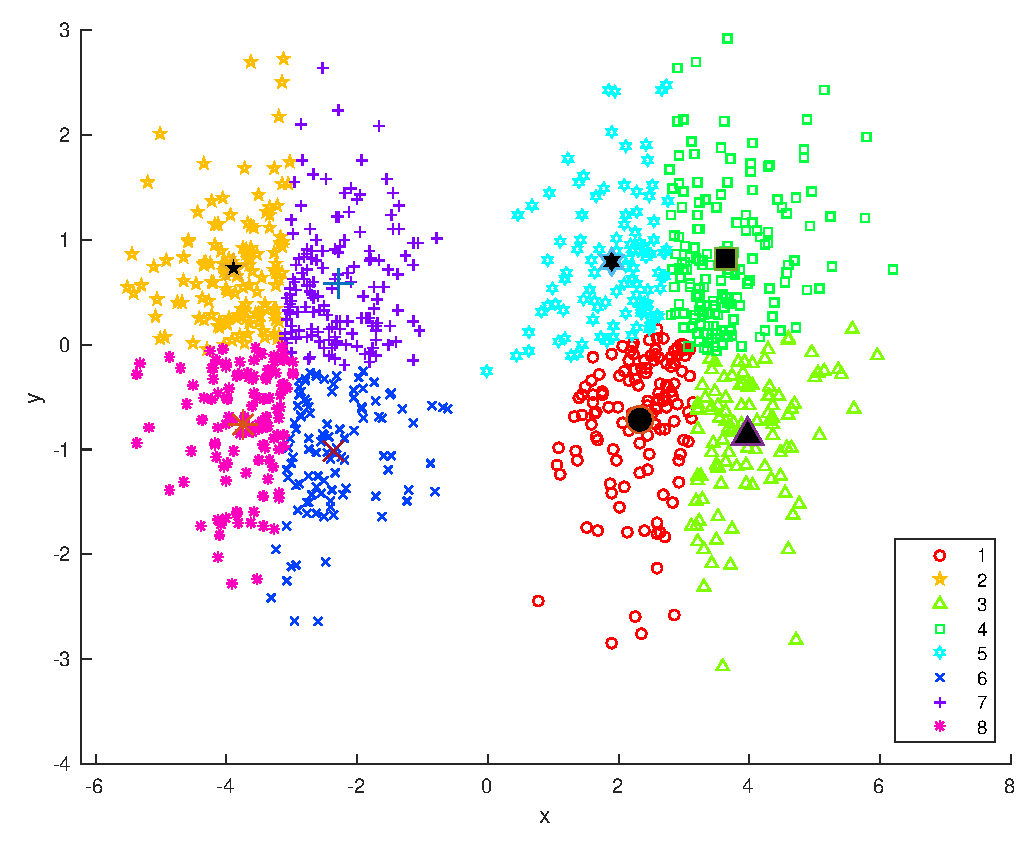
\includegraphics[width=\columnwidth]{Fig2_k8.eps}
    \caption{The final cluster means with their assigned data points)}
  \end{subfigure}
  \label{fig1.3}
\end{figure}

\noindent We (humans) can clearly see that the data form two clusters. Therefore figure \ref{fig1a}, which has a $k$ of 2, shows the quickest convergence to the final cluster centers. Usually it takes about two epochs for the cluster centers to converge, as is shown in the figure. Figure \ref{fig1b} shows that these centers form in the places which the human eye observes to be the correct centers. When we choose $k$ as 4, as shown in figure \ref{fig1.2}, we can see that, dependent on the initialization, sometimes one main cluster gets divided into three subclusters and the other remains one cluster, and sometimes the two clusters get separated into two clusters each. The number of epochs it takes to reach convergence is high compared to a run using $k=2$. This can be explained by the fact that the data are not naturally separated into four clusters but in two, so the distances between the data points within a main cluster are small. This causes the algorithm to take longer to find a convergence, since the cluster centers switch often during the clustering process. Finally figure \ref{fig1.3} shows the clustering for $k = 8$, which takes the longest amount of epochs to converge, because of the same reasoning. It separates both of the clusters into four subclusters. 

\subsection{}
Using the code given in the appendix (kmeans.m and runKMeans.m) we computed the quantization errors and D-function given in figure \ref{fig2.1}.

\begin{figure}[H]
  \centering
  \caption{Results for $kmax = 20$. The triangles give $k_{opt}$}
  \begin{subfigure}[b]{.45\textwidth}
    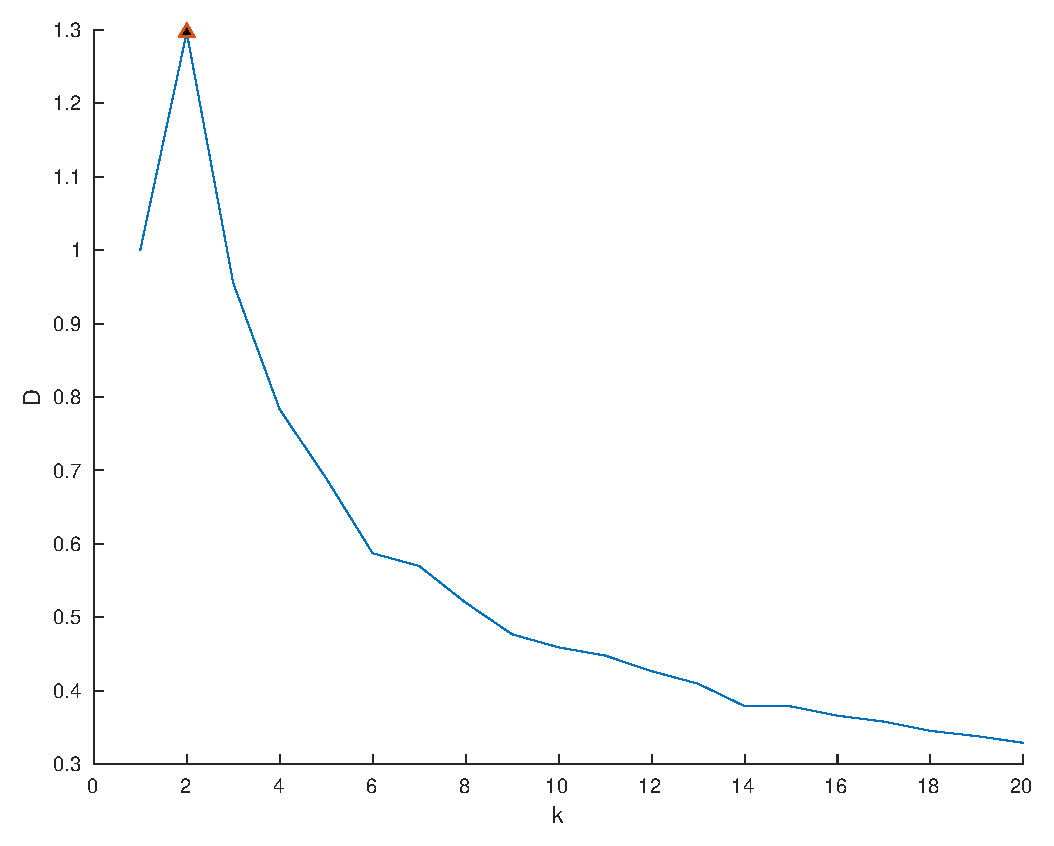
\includegraphics[width=\columnwidth]{Fig3.eps}
    \caption{The D-function.}
  \end{subfigure}
  \quad
  \begin{subfigure}[b]{.45\textwidth}
    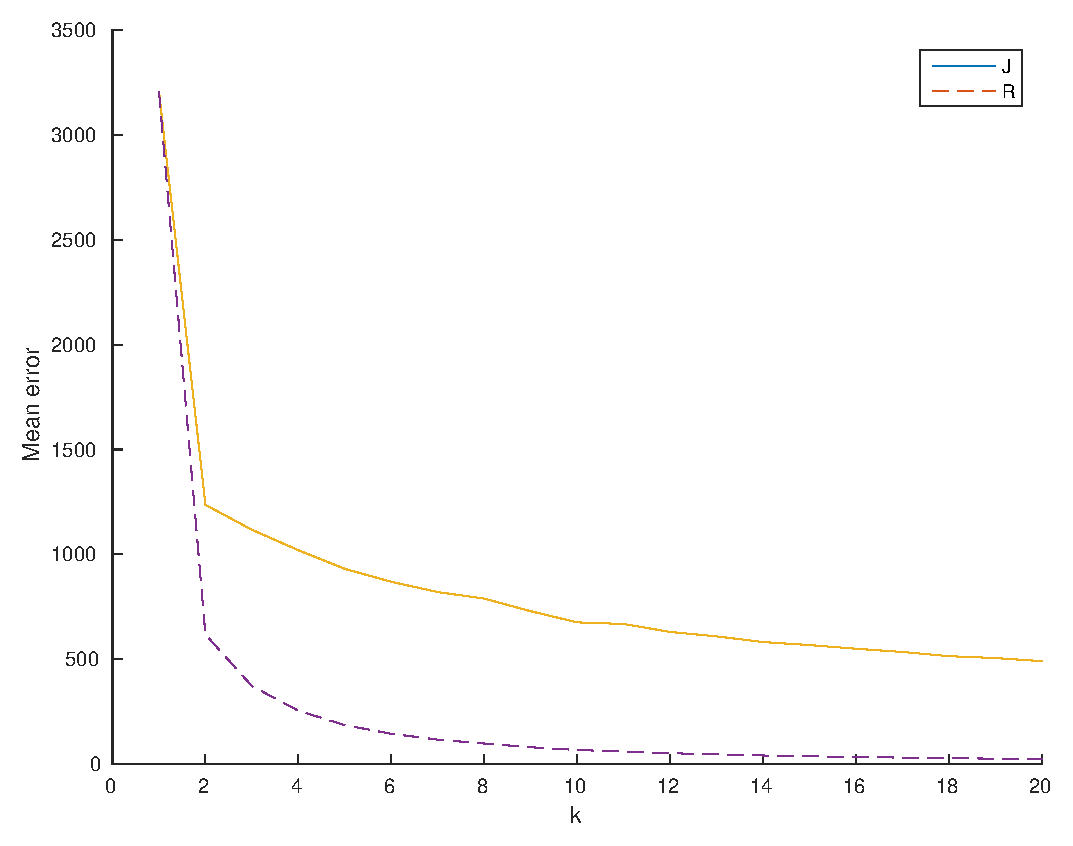
\includegraphics[width=\columnwidth]{Fig4.eps}
    \caption{The quantization error function $J(k)$ and the reference function $R(k)$.}
  \end{subfigure}
  \label{fig2.1}
\end{figure}

\noindent Figure \ref{fig2.1} shows the $D(k)$, $J(k)$ and $R(k)$ for a $kmax$ of 20. Here $k_{opt} = \argmax_k D(k)$ is the $k$ for which the difference between the error function and the reference function is the largest. Figure \ref{fig2.1} shows that $k_{opt}$ can be found at a $k$ of 2, which was expected because it could clearly be seen by a human that the data are divided into two main clusters. $D(k)$ decreases as $k$ increases, clusters that have no natural division need to be divided by even more clusters, which causes them to shift a lot before finally reaching convergence.

\subsection{}
\subsubsection{}
See the part in kmeans.m which is commented ``Kmeans plusplus initialization''.

\subsubsection{}
We computed the following means and standard deviations given in \ref{tab1}.
\begin{table}[H]
 \centering
 \caption{Mean and standard deviation of quantization error for $k = 100$.}
 \begin{tabular}{c|c|c}
  Algorithm & mean q-error & sd q-error \\
  \hline
  $kmeans++$ & 10.0310 & 0.3502 \\
  $kmeans$ & 10.6001 & 0.4268 
 \end{tabular}
 \label{tab1}
\end{table}

\subsubsection{}
We calculated the following p-value using a an unpaired one-tailed two-sample t-test (see runKMeans.m at the bottom): $2.3816e^{-5}$. This p-value is significant (<0.05), which means that we have enough certainty to reject the null hypothesis that there is no difference in performance between the two algorithmes. Hence, we assume a difference between the performance of the two algorithmes ($kmeans++$ performs better).

\section{Batch Neural gas vs k-means}
\subsection{}
Code batchNG.m in the appendix gives our implementation of the Neural gas algorithm.

\subsection{}

\subsection{}


\section*{Appendix}
\lstinputlisting{../Code/kmeans.m}{\label{kmeans}}
\lstinputlisting{../Code/runKMeans.m}{\label{runKMeans}}

\end{document}
